\chapter{从导论课走向磁重联：先建立一张可计算的地图}
\label{hall:orientation}
\section{这份讲义要让你真正会做什么}
导论课已经告诉我们：带电粒子受洛伦兹力，粒子会回旋，等离子体能够屏蔽电场，也能支持各种波。现在的问题是：数以亿计的粒子共同形成一层很薄的电流片时，磁场为什么会改变连接方式？离子与电子是否仍能被看成一团共同运动的物质？哪条方程告诉我们模型失效了？

本讲义把这些问题转成五项可练习的能力：能从分布函数推导物种方程；能说明每次约化删掉了哪项和为什么能删；能用实际数字比较欧姆定律各项；能从磁通、能量和尺度判断某个重联图像是否自洽；能看懂一篇Hall或双流体论文究竟求解了什么。所有主要数量级例题均给出计算过程和结论，不把关键步骤留给读者补。

\note{第一次阅读可以先读本章，然后连续读第2--5章掌握方程来源；第7章的数字算例应逐行跟算。第8章把方程放回重联层，第9章用波检验Hall项，第10章讨论模拟与证据。第11章含有完整答案，用来检查是否真正掌握。}

\section{同一等离子体的三个描述层次}
\paragraph{粒子层次。}每个电子都服从$m_e\dd\vct v/\dd t=-e(\E+\vct v\times\B)$。若直接跟踪全部真实粒子，变量太多；粒子模拟也只是以数值粒子抽样分布。
\paragraph{分布函数层次。}$f_s(\vct x,\vct v,t)\dd^3x\dd^3v$表示位置和速度小体积中的粒子数。它能区分向右运动的一束和向左运动的一束，即使两束的平均速度为零。
\paragraph{流体层次。}把速度空间积分，得到密度、平均速度、压力及热流。电子是一套，离子是一套，便是本文的\emph{电子--离子双流体}。双流体并不是两种互不相干的液体：两者通过同一电磁场和碰撞强烈耦合。

理想MHD进一步以近似共同的整体运动描述两者。Hall MHD则保留电子和离子之间对磁通输运重要的相对运动。它常写成一套总动量方程加一条广义欧姆定律，外观像单流体，但仍含两物种的差异。因此“方程里只有一个显式速度演化式”不能用来判断是否保留了双流体物理。

\section{单位、温度和坐标：先约定，后计算}
全文采用SI单位。$e=1.602176634\times10^{-19}\,\mathrm C$是\emph{正}的元电荷，离子电荷$+e$，电子电荷$-e$。默认离子为质子，质量$m_i=1.67262\times10^{-27}\,\mathrm{kg}$；电子质量$m_e=9.10938\times10^{-31}\,\mathrm{kg}$。氘或多电荷离子需要重新代入质量与电荷，不能沿用所有氢的数值。

用$\Theta_s=k_BT_{s,\mathrm K}$表示以焦耳为单位的温度能量，故标量压强$p_s=n_s\Theta_s$。若实验写$T_s=20\,\mathrm{eV}$，计算时用
\begin{equation}
\Theta_s=e\,(20\,\mathrm V)=3.20435\times10^{-18}\,\mathrm J,
\end{equation}
通常简写为$\Theta_s=eT_s$，这里$T_s$指以eV报告的数值。不要再乘一次$k_B$。热速度约定为$v_{ts}=\sqrt{2\Theta_s/m_s}$；有些教材用不含2的定义，所以比较回旋半径和碰撞平均自由程前应先对齐约定。

电阻率写$\eta$，单位$\Omega\,\mathrm m$；磁扩散系数写$D_\eta=\eta/\mu_0$，单位$\mathrm{m^2/s}$。文献常把两者都叫$\eta$，但本讲义不混用。$\Omega_s$是角频率，单位$\mathrm{s^{-1}}$；普通频率$f_s=|\Omega_s|/(2\pi)$，二者不能少除一个$2\pi$。

二维重联采用$x$为出流方向、$y$为入流方向、$z$为面外电流/导场方向。图\ref{hall:figgeometry}中的磁力线是解析示意，不是模拟或实测。伴随讲义Lecture-TM采用另一常见约定$x$跨片、$y$沿片；两份讲义的物理相同，但不要直接照搬分量下标。
\begin{figure}[htbp]\centering
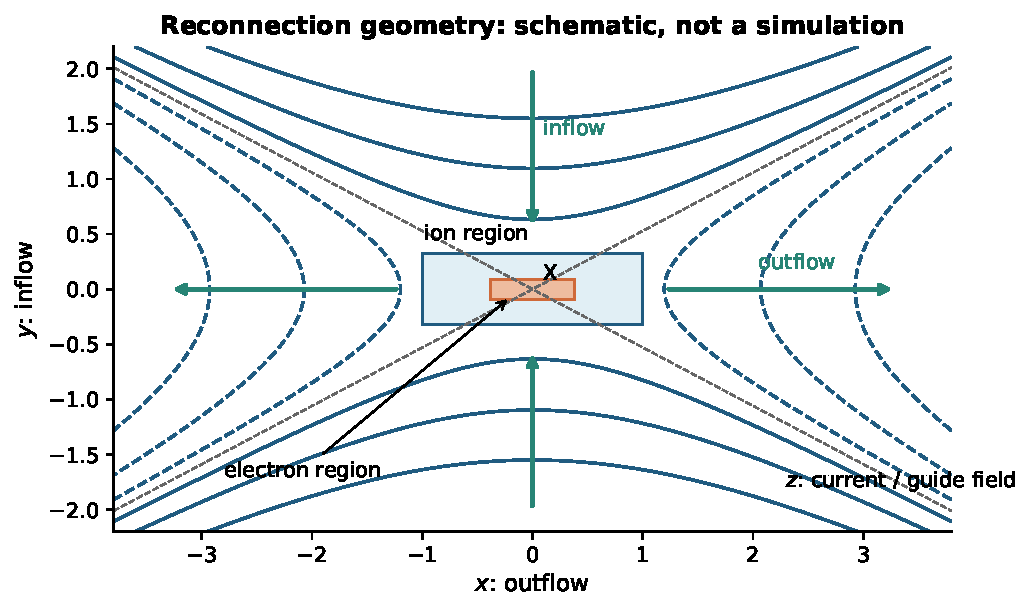
\includegraphics[width=.94\textwidth]{figures/01_geometry.pdf}
\caption{重联几何及两个内层的示意。蓝色等值线来自$A_z=(y^2-0.28x^2)/2$；矩形仅表示尺度层次，不表示真实层宽或层长比。绿色箭头为入流与出流，真实解须同时满足连续性、动量和磁通约束。}\label{hall:figgeometry}
\end{figure}

\section{磁力线、磁通与“断线”分别指什么}
磁力线是在\emph{同一时刻}处处与$\B$相切的曲线，满足$\dd\vct x/\dd l\parallel\B$；它不是一根有材料编号的橡皮绳。所谓磁场连接关系，是场线从一个区域进入、沿磁场到达哪个区域的映射。重联讨论这个映射怎样随时间改变，而不是用肉眼判断两条线是否在画面上相交。

二维$\partial_z=0$时可写
\begin{equation}
\B_\perp=\nabla A_z\times\hat{\vct z}
=(\partial_yA_z,-\partial_xA_z,0),\qquad
\B_\perp\cdot\nabla A_z=0.
\end{equation}
所以$A_z$的等值线就是面内磁力线。相邻等值线的$\Delta A_z$表示单位$z$长度的磁通，单位是$\mathrm{T\,m= Wb/m}$。它不是磁场强度，量纲比$B$多一个长度。

X点是$A_z$的鞍点：两个方向曲率符号相反；O点是局地极大或极小点，周围有闭合等值线形成磁岛。分离线经过X点，区分不同连接区域。三维里没有一个标量$A_z$能替代全部场线拓扑；不能把二维X点公式不加说明地直接套到三维。

\section{一个电流片为什么能够静止：Harris型力平衡}
先不谈重联，构造静态平衡。设
\begin{equation}
\B=B_x(y)\hat{\vct x}+B_g\hat{\vct z},\qquad B_x=B_0\tanh(y/a),
\end{equation}
$a$为半厚度，$B_g$为常数导场。忽略位移电流，逐分量求旋度：
\begin{equation}
\J=\frac{\nabla\times\B}{\mu_0}
=-\frac{B_0}{\mu_0a}\operatorname{sech}^2(y/a)\hat{\vct z}.
\end{equation}
由于$\hat{\vct z}\times\hat{\vct x}=\hat{\vct y}$，洛伦兹力的$y$分量为$J_zB_x=-B_x\partial_yB_x/\mu_0$。静态总动量平衡$0=-\nabla p+\J\times\B$给
\begin{align}
\frac{\dd p}{\dd y}&=-\frac{B_x}{\mu_0}\frac{\dd B_x}{\dd y},\\
\frac{\dd}{\dd y}\left(p+\frac{B_x^2}{2\mu_0}\right)&=0,\\
p(y)&=p_\infty+\frac{B_0^2}{2\mu_0}\operatorname{sech}^2(y/a).
\end{align}
导场为常数，其磁压也为常数，因此不出现在梯度中。电流片中间反向磁场减弱，总热压必须增加以补偿。这个压力可以由更高密度、更高温度或二者共同提供，不能只凭平衡式唯一决定。
\begin{figure}[htbp]\centering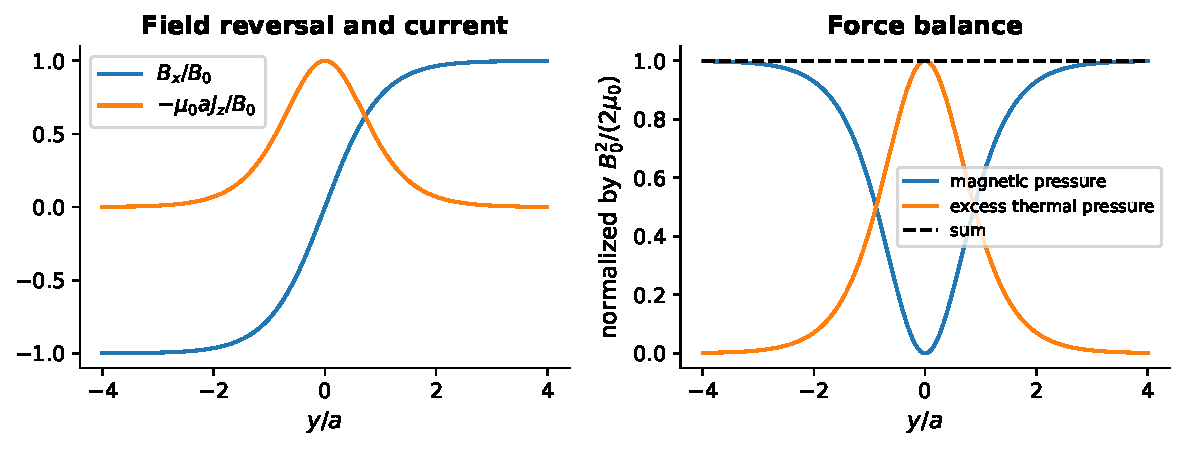
\includegraphics[width=\textwidth]{figures/02_harris.pdf}
\caption{Harris型平衡的解析曲线。左图电流取负号后与$\operatorname{sech}^2$同号；右图显示增加的热压与反向磁场的磁压之和恒定。此图检验静态力平衡，不表示重联已经发生。}\label{hall:figharris}\end{figure}

\worked{已算例：电流并不要求大量电荷分离}
取$B_0=0.05\,\mathrm T$、$a=0.01\,\mathrm m$、中心密度$n=10^{19}\,\mathrm{m^{-3}}$。中心电流绝对值
\begin{equation}
|J_z(0)|=\frac{0.05}{(1.25664\times10^{-6})(0.01)}
=3.98\times10^6\,\mathrm{A/m^2}.
\end{equation}
即使$n_i=n_e=n$，仍有
\begin{equation}
|u_{iz}-u_{ez}|=\frac{|J_z|}{en}
=\frac{3.98\times10^6}{(1.60218\times10^{-19})(10^{19})}
=2.48\times10^6\,\mathrm{m/s}.
\end{equation}
电荷密度$e(n_i-n_e)$为零，而电流不为零，因为电子和离子的\emph{通量}不同。本例只给了总流差；由电子承担多少，需要额外初始条件。若把它全部分配给电子，应另外检查其漂移能和可能的流致不稳定性。

\section{一张模型选择表，以及两个需要避免的误解}
\begin{longtable}{P{25mm}P{51mm}P{70mm}}
\toprule 模型 & 保留的主要信息 & 一开始就该问的问题\\\midrule\endfirsthead
\toprule 模型 & 保留的主要信息 & 一开始就该问的问题\\\midrule\endhead
理想MHD & 总体流动，理想磁通冻结 & 目标层厚是否远大于非MHD尺度？是否需要改变磁连接？\\
电阻MHD & 总体运动与电阻磁扩散 & 电阻来自什么碰撞/模型？层内是否仍适用流体闭合？\\
Hall MHD & 离子/总体流与电子磁通输运不同 & 电子层由什么破冻结？电子压强及热流怎样闭合？\\
惯性扩展 & 增加电子惯性/相对流能 & 保留的惯性与总能量是否一致？是否使用准中性？\\
五矩双流体 & 两套密度、动量、标量能量 & 是否需要各向异性/非对角压力？电磁方程取何约化？\\
十矩双流体 & 两套对称压力张量 & 三阶热流怎么关？压力是否正定，闭合有无校准依赖？\\
\bottomrule\end{longtable}
“双流体”是物种划分，“五矩/十矩”是保留的速度矩阶数，“准中性/全Maxwell”是电磁约化；它们不是同一条线上的互斥选项。第二个误解是“更复杂一定更准确”。复杂方程若闭合、边界或网格不合适，也会给出错误温度和电场。我们将反复区分数学上\emph{能表示}一个量、数值上\emph{算得收敛}和物理上\emph{通过观测}这三件事。\citep{Birn2001,Wang2015}
